
\section{Experiments}
\label{seq:experiments}

\noindent All data modules live at \url{https://github.com/krzysztof-turowski/string-algorithms}.

\subsection{Runs}
All texts come from the generators that ship with the \texttt{string-algorithms} repository, so that the experiments can be reproduced without any additional data. 
Four modules are used:
\begin{itemize}
    \item \texttt{generator/named.py} for the two morphic words,
    \item \texttt{generator/rand.py} 
    \item \texttt{generator/input/pantadeusz.txt} example of real text, 
    \item \texttt{generator/exact\_string\_matching.py} for worst case.
\end{itemize}



\begin{table}[H]
\centering
\begin{tabular}{lp{6.0cm}p{5.5cm}r}
\hline
text & description & generator & $\alpha$ \\
\hline
Fibonacci & the Fibonacci word & fibonacci\_word & 2 \\
Thue-Morse & the Thue-Morse word & thue\_word & 2 \\
random binary & uniform over two letters & random\_word & 2 \\
random 26 & uniform over the lowercase Latin alphabet & random\_word & 26 \\
natural & Pan Tadeusz & natural\_generator & 33 \\
\hline
\end{tabular}
\caption{Texts used in the experiments.}
\label{tab:texts}
\end{table}

Every text is truncated to the same length $n$, so that the rows of one table are directly comparable. Each algorithm runs in its \emph{OFFLINE} configuration, with the whole text available from start.

% {
% \setlength{\floatsep}{6pt plus 2pt minus 2pt}
% \setlength{\textfloatsep}{6pt plus 2pt minus 2pt}
% \setlength{\intextsep}{6pt plus 2pt minus 2pt}
% \setlength{\abovecaptionskip}{4pt}
% \setlength{\belowcaptionskip}{0pt}

% \input{chapters/ComparisonAndExperiments/tables/tables}
% }
Each table reports, for one text and all four implementations:
\begin{itemize}
    \item \(n\) --- length of source
    \item \(\alpha\) --- size of alphabet
    \item \(z\) --- the number of codewords produced by algorithm
    \item \(\rho\) --- the compression ratio, computed according to \Cref{def:compression-ratio}.
    \item \texttt{encode} --- working time of encoder in ms
    \item \texttt{decode} --- working time of decoder in ms
\end{itemize}

\subsubsection{Fibonacci}
 {
\setlength{\floatsep}{6pt plus 2pt minus 2pt}
\setlength{\textfloatsep}{6pt plus 2pt minus 2pt}
\setlength{\intextsep}{6pt plus 2pt minus 2pt}
\setlength{\abovecaptionskip}{4pt}
\setlength{\belowcaptionskip}{0pt}

\begin{center}
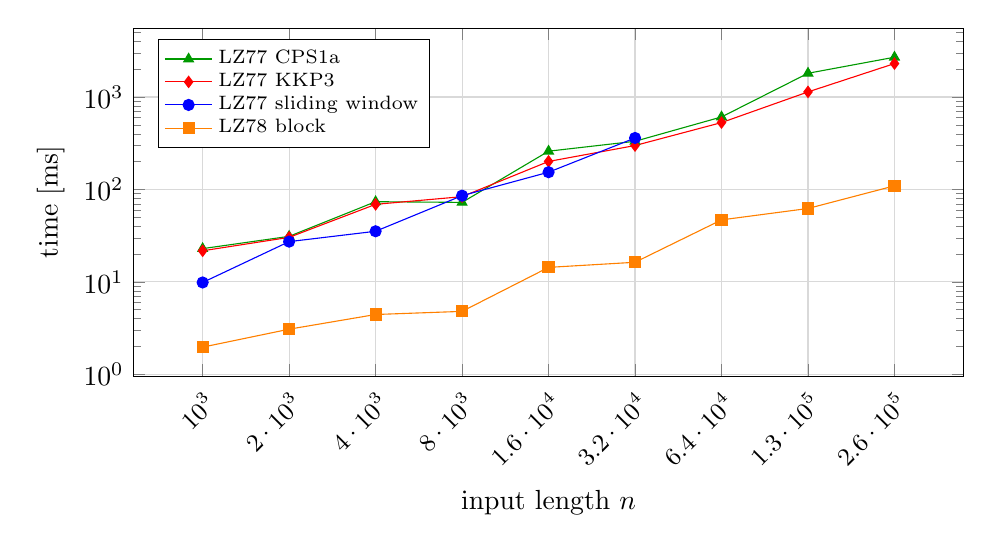
\begin{tikzpicture}
\begin{axis}[
  width = \linewidth, height = 6cm,
  xlabel = {input length $n$}, ylabel = {time [ms]},
  xmode = log, ymode = log,
  legend pos = north west, legend cell align = left,
  legend style = {font = \scriptsize, row sep = -2pt, inner sep = 2pt},
  xmajorgrids = true, ymajorgrids = true,
  xminorgrids = false, yminorgrids = false,
  minor tick num = 0,
  grid style = {draw = gray!30},
  xtick = {1000, 2000, 4000, 8000, 16000, 32000, 64000, 128000, 256000},
  xticklabels = {$10^{3}$, $2 \cdot 10^{3}$, $4 \cdot 10^{3}$, $8 \cdot 10^{3}$, $1.6 \cdot 10^{4}$, $3.2 \cdot 10^{4}$, $6.4 \cdot 10^{4}$, $1.3 \cdot 10^{5}$, $2.6 \cdot 10^{5}$},
  x tick label style = {rotate = 45, anchor = north east, font = \small},
]
\addplot[color = green!60!black, mark = triangle*] coordinates {(1000, 22.91) (2000, 31.1) (4000, 73.73) (8000, 72.49) (16000, 259.4) (32000, 331.96) (64000, 608.61) (128000, 1806.19) (256000, 2694.28)};
\addlegendentry{LZ77 CPS1a}
\addplot[color = red, mark = diamond*] coordinates {(1000, 21.71) (2000, 30.33) (4000, 69.04) (8000, 83.58) (16000, 200.89) (32000, 298.71) (64000, 528.87) (128000, 1135.06) (256000, 2299.99)};
\addlegendentry{LZ77 KKP3}
\addplot[color = blue, mark = *] coordinates {(1000, 9.86) (2000, 27.27) (4000, 35.3) (8000, 85.68) (16000, 153.7) (32000, 360.45)};
\addlegendentry{LZ77 sliding window}
\addplot[color = orange, mark = square*] coordinates {(1000, 1.97) (2000, 3.08) (4000, 4.44) (8000, 4.8) (16000, 14.36) (32000, 16.31) (64000, 46.87) (128000, 62.27) (256000, 109.43)};
\addlegendentry{LZ78 block}
\end{axis}
\end{tikzpicture}
\captionof{figure}{Fibonacci, encoding time.}
\label{fig:Fibonacci-encoding}
\end{center}

\begin{center}
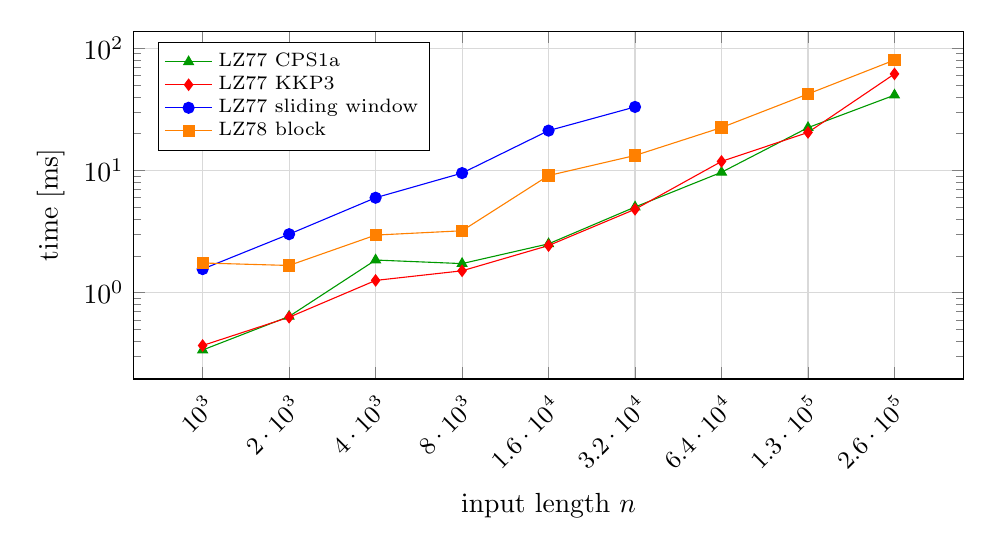
\begin{tikzpicture}
\begin{axis}[
  width = \linewidth, height = 6cm,
  xlabel = {input length $n$}, ylabel = {time [ms]},
  xmode = log, ymode = log,
  legend pos = north west, legend cell align = left,
  legend style = {font = \scriptsize, row sep = -2pt, inner sep = 2pt},
  xmajorgrids = true, ymajorgrids = true,
  xminorgrids = false, yminorgrids = false,
  minor tick num = 0,
  grid style = {draw = gray!30},
  xtick = {1000, 2000, 4000, 8000, 16000, 32000, 64000, 128000, 256000},
  xticklabels = {$10^{3}$, $2 \cdot 10^{3}$, $4 \cdot 10^{3}$, $8 \cdot 10^{3}$, $1.6 \cdot 10^{4}$, $3.2 \cdot 10^{4}$, $6.4 \cdot 10^{4}$, $1.3 \cdot 10^{5}$, $2.6 \cdot 10^{5}$},
  x tick label style = {rotate = 45, anchor = north east, font = \small},
]
\addplot[color = green!60!black, mark = triangle*] coordinates {(1000, 0.34) (2000, 0.64) (4000, 1.85) (8000, 1.73) (16000, 2.51) (32000, 5.02) (64000, 9.66) (128000, 22.39) (256000, 41.29)};
\addlegendentry{LZ77 CPS1a}
\addplot[color = red, mark = diamond*] coordinates {(1000, 0.37) (2000, 0.63) (4000, 1.26) (8000, 1.51) (16000, 2.43) (32000, 4.81) (64000, 11.85) (128000, 20.46) (256000, 61.55)};
\addlegendentry{LZ77 KKP3}
\addplot[color = blue, mark = *] coordinates {(1000, 1.56) (2000, 3.01) (4000, 5.98) (8000, 9.51) (16000, 21.16) (32000, 33.06)};
\addlegendentry{LZ77 sliding window}
\addplot[color = orange, mark = square*] coordinates {(1000, 1.75) (2000, 1.67) (4000, 2.96) (8000, 3.21) (16000, 9.08) (32000, 13.25) (64000, 22.42) (128000, 42.2) (256000, 79.93)};
\addlegendentry{LZ78 block}
\end{axis}
\end{tikzpicture}
\captionof{figure}{Fibonacci, decoding time.}
\label{fig:Fibonacci-decoding}
\end{center}

\begin{center}
\begin{tabular}{lrrrrrr}
\hline
algorithm & $n$ & $\alpha$ & $z$ & $\rho$ & encode [ms] & decode [ms] \\
\hline
LZ77 sliding window & 32000 & 2 & 22 & 0.0213 & 469.08 & 64.52 \\
LZ78 block & 32000 & 2 & 1050 & 0.3298 & 152.9 & 35.42 \\
LZ77 CPS1a & 32000 & 2 & 22 & 0.0206 & 605.42 & 8.11 \\
LZ77 KKP3 & 32000 & 2 & 22 & 0.0206 & 545.25 & 10.96 \\
\hline
\end{tabular}
\captionof{table}{Fibonacci: the Fibonacci word.}
\label{tab:Fibonacci}
\end{center}

}

\subsubsection{Thue-Morse}
{
\setlength{\floatsep}{6pt plus 2pt minus 2pt}
\setlength{\textfloatsep}{6pt plus 2pt minus 2pt}
\setlength{\intextsep}{6pt plus 2pt minus 2pt}
\setlength{\abovecaptionskip}{4pt}
\setlength{\belowcaptionskip}{0pt}

\begin{center}
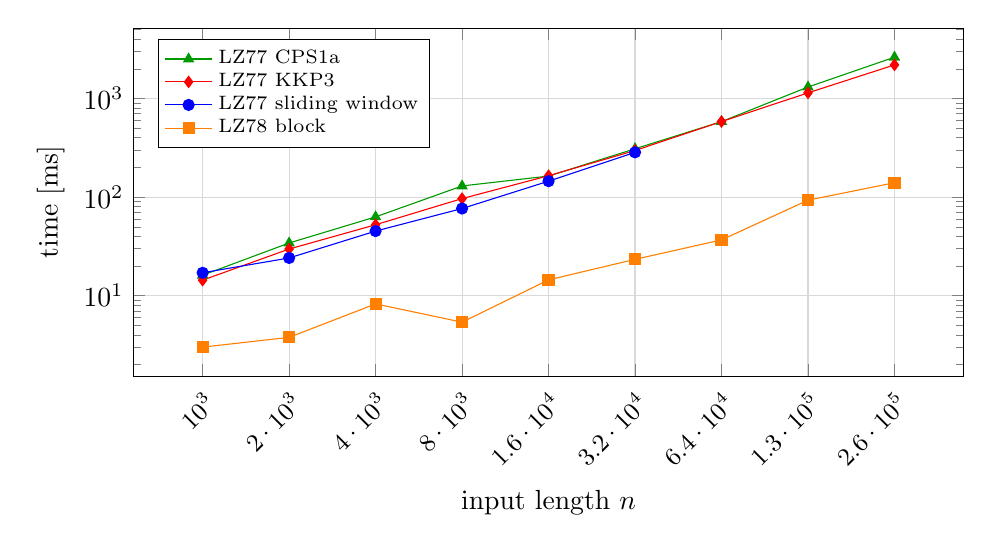
\begin{tikzpicture}
\begin{axis}[
  width = \linewidth, height = 6cm,
  xlabel = {input length $n$}, ylabel = {time [ms]},
  xmode = log, ymode = log,
  legend pos = north west, legend cell align = left,
  legend style = {font = \scriptsize, row sep = -2pt, inner sep = 2pt},
  xmajorgrids = true, ymajorgrids = true,
  xminorgrids = false, yminorgrids = false,
  minor tick num = 0,
  grid style = {draw = gray!30},
  xtick = {1000, 2000, 4000, 8000, 16000, 32000, 64000, 128000, 256000},
  xticklabels = {$10^{3}$, $2 \cdot 10^{3}$, $4 \cdot 10^{3}$, $8 \cdot 10^{3}$, $1.6 \cdot 10^{4}$, $3.2 \cdot 10^{4}$, $6.4 \cdot 10^{4}$, $1.3 \cdot 10^{5}$, $2.6 \cdot 10^{5}$},
  x tick label style = {rotate = 45, anchor = north east, font = \small},
]
\addplot[color = green!60!black, mark = triangle*] coordinates {(1000, 16.14) (2000, 34.24) (4000, 63.02) (8000, 129.76) (16000, 163.47) (32000, 309.23) (64000, 582.9) (128000, 1307.41) (256000, 2622.61)};
\addlegendentry{LZ77 CPS1a}
\addplot[color = red, mark = diamond*] coordinates {(1000, 14.38) (2000, 29.74) (4000, 52.43) (8000, 96.62) (16000, 164.66) (32000, 296.95) (64000, 583.29) (128000, 1140.96) (256000, 2190.97)};
\addlegendentry{LZ77 KKP3}
\addplot[color = blue, mark = *] coordinates {(1000, 17.09) (2000, 24.14) (4000, 45.24) (8000, 76.6) (16000, 145.07) (32000, 284.37)};
\addlegendentry{LZ77 sliding window}
\addplot[color = orange, mark = square*] coordinates {(1000, 3.01) (2000, 3.78) (4000, 8.26) (8000, 5.39) (16000, 14.47) (32000, 23.38) (64000, 36.82) (128000, 93.05) (256000, 139.94)};
\addlegendentry{LZ78 block}
\end{axis}
\end{tikzpicture}
\captionof{figure}{Thue-Morse, encoding time.}
\label{fig:Thue-Morse-encoding}
\end{center}

\begin{center}
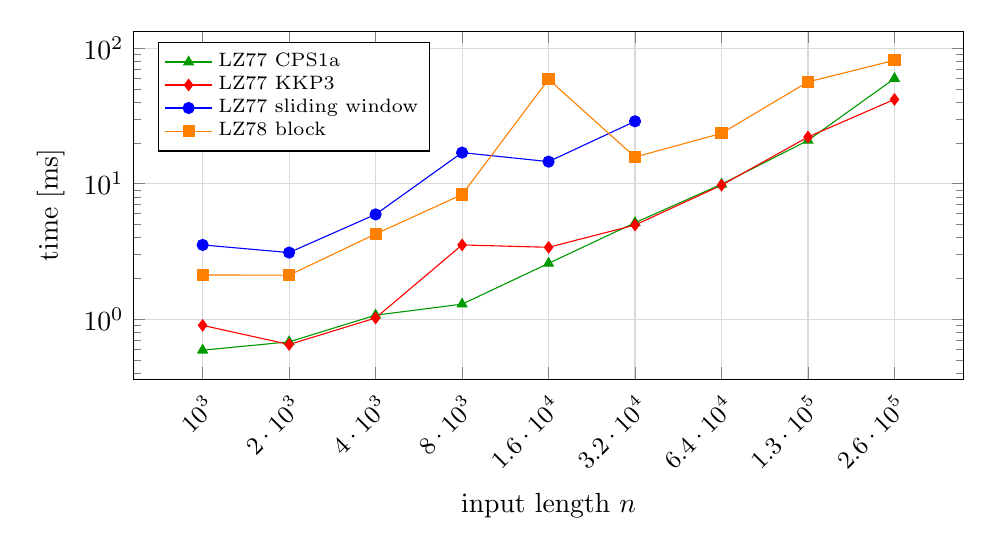
\begin{tikzpicture}
\begin{axis}[
  width = \linewidth, height = 6cm,
  xlabel = {input length $n$}, ylabel = {time [ms]},
  xmode = log, ymode = log,
  legend pos = north west, legend cell align = left,
  legend style = {font = \scriptsize, row sep = -2pt, inner sep = 2pt},
  xmajorgrids = true, ymajorgrids = true,
  xminorgrids = false, yminorgrids = false,
  minor tick num = 0,
  grid style = {draw = gray!30},
  xtick = {1000, 2000, 4000, 8000, 16000, 32000, 64000, 128000, 256000},
  xticklabels = {$10^{3}$, $2 \cdot 10^{3}$, $4 \cdot 10^{3}$, $8 \cdot 10^{3}$, $1.6 \cdot 10^{4}$, $3.2 \cdot 10^{4}$, $6.4 \cdot 10^{4}$, $1.3 \cdot 10^{5}$, $2.6 \cdot 10^{5}$},
  x tick label style = {rotate = 45, anchor = north east, font = \small},
]
\addplot[color = green!60!black, mark = triangle*] coordinates {(1000, 0.59) (2000, 0.68) (4000, 1.07) (8000, 1.29) (16000, 2.58) (32000, 5.15) (64000, 9.9) (128000, 20.85) (256000, 59.68)};
\addlegendentry{LZ77 CPS1a}
\addplot[color = red, mark = diamond*] coordinates {(1000, 0.9) (2000, 0.65) (4000, 1.02) (8000, 3.53) (16000, 3.39) (32000, 4.95) (64000, 9.74) (128000, 22.11) (256000, 41.88)};
\addlegendentry{LZ77 KKP3}
\addplot[color = blue, mark = *] coordinates {(1000, 3.53) (2000, 3.1) (4000, 5.93) (8000, 16.95) (16000, 14.54) (32000, 28.85)};
\addlegendentry{LZ77 sliding window}
\addplot[color = orange, mark = square*] coordinates {(1000, 2.12) (2000, 2.11) (4000, 4.25) (8000, 8.31) (16000, 58.87) (32000, 15.72) (64000, 23.51) (128000, 56.39) (256000, 81.38)};
\addlegendentry{LZ78 block}
\end{axis}
\end{tikzpicture}
\captionof{figure}{Thue-Morse, decoding time.}
\label{fig:Thue-Morse-decoding}
\end{center}

\begin{center}
\begin{tabular}{lrrrrrr}
\hline
algorithm & $n$ & $\alpha$ & $z$ & $\rho$ & encode [ms] & decode [ms] \\
\hline
LZ77 sliding window & 32000 & 2 & 29 & 0.0281 & 461.67 & 49.65 \\
LZ78 block & 32000 & 2 & 1425 & 0.4704 & 29.4 & 26.28 \\
LZ77 CPS1a & 32000 & 2 & 29 & 0.0263 & 448.91 & 8.45 \\
LZ77 KKP3 & 32000 & 2 & 29 & 0.0263 & 410.0 & 8.69 \\
\hline
\end{tabular}
\captionof{table}{Thue-Morse: the Thue-Morse word.}
\label{tab:Thue-Morse}
\end{center}
}

\subsubsection{Random 26}
{
\setlength{\floatsep}{6pt plus 2pt minus 2pt}
\setlength{\textfloatsep}{6pt plus 2pt minus 2pt}
\setlength{\intextsep}{6pt plus 2pt minus 2pt}
\setlength{\abovecaptionskip}{4pt}
\setlength{\belowcaptionskip}{0pt}

\begin{center}
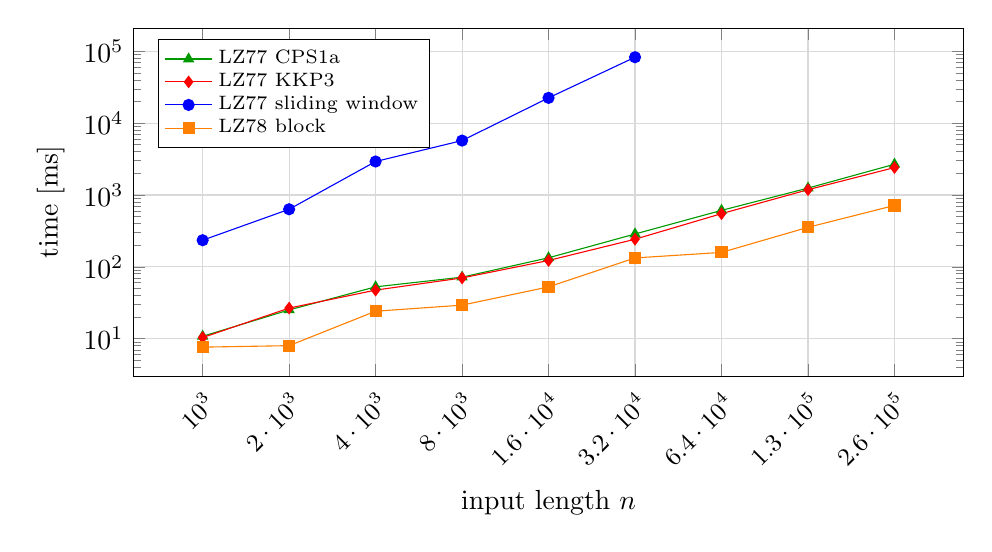
\begin{tikzpicture}
\begin{axis}[
  width = \linewidth, height = 6cm,
  xlabel = {input length $n$}, ylabel = {time [ms]},
  xmode = log, ymode = log,
  legend pos = north west, legend cell align = left,
  legend style = {font = \scriptsize, row sep = -2pt, inner sep = 2pt},
  xmajorgrids = true, ymajorgrids = true,
  xminorgrids = false, yminorgrids = false,
  minor tick num = 0,
  grid style = {draw = gray!30},
  xtick = {1000, 2000, 4000, 8000, 16000, 32000, 64000, 128000, 256000},
  xticklabels = {$10^{3}$, $2 \cdot 10^{3}$, $4 \cdot 10^{3}$, $8 \cdot 10^{3}$, $1.6 \cdot 10^{4}$, $3.2 \cdot 10^{4}$, $6.4 \cdot 10^{4}$, $1.3 \cdot 10^{5}$, $2.6 \cdot 10^{5}$},
  x tick label style = {rotate = 45, anchor = north east, font = \small},
]
\addplot[color = green!60!black, mark = triangle*] coordinates {(1000, 10.79) (2000, 25.11) (4000, 52.62) (8000, 71.76) (16000, 133.5) (32000, 286.24) (64000, 610.1) (128000, 1246.03) (256000, 2676.51)};
\addlegendentry{LZ77 CPS1a}
\addplot[color = red, mark = diamond*] coordinates {(1000, 10.36) (2000, 26.63) (4000, 47.39) (8000, 70.0) (16000, 122.47) (32000, 241.99) (64000, 549.13) (128000, 1183.11) (256000, 2405.25)};
\addlegendentry{LZ77 KKP3}
\addplot[color = blue, mark = *] coordinates {(1000, 234.39) (2000, 632.04) (4000, 2921.45) (8000, 5712.69) (16000, 22457.89) (32000, 82635.17)};
\addlegendentry{LZ77 sliding window}
\addplot[color = orange, mark = square*] coordinates {(1000, 7.62) (2000, 7.99) (4000, 24.09) (8000, 29.27) (16000, 52.51) (32000, 132.83) (64000, 158.65) (128000, 354.64) (256000, 714.29)};
\addlegendentry{LZ78 block}
\end{axis}
\end{tikzpicture}
\captionof{figure}{random 26, encoding time.}
\label{fig:random-26-encoding}
\end{center}

\begin{center}
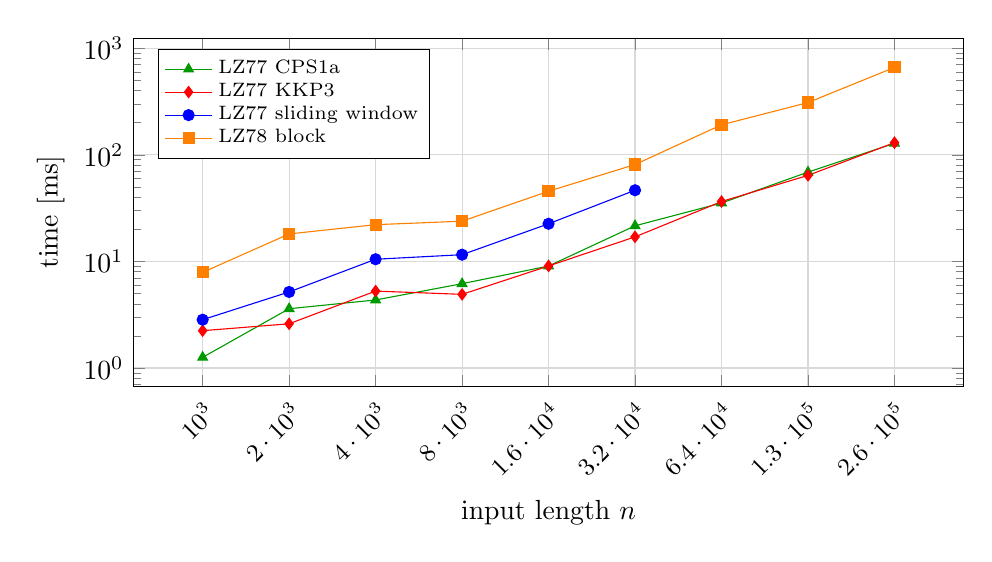
\begin{tikzpicture}
\begin{axis}[
  width = \linewidth, height = 6cm,
  xlabel = {input length $n$}, ylabel = {time [ms]},
  xmode = log, ymode = log,
  legend pos = north west, legend cell align = left,
  legend style = {font = \scriptsize, row sep = -2pt, inner sep = 2pt},
  xmajorgrids = true, ymajorgrids = true,
  xminorgrids = false, yminorgrids = false,
  minor tick num = 0,
  grid style = {draw = gray!30},
  xtick = {1000, 2000, 4000, 8000, 16000, 32000, 64000, 128000, 256000},
  xticklabels = {$10^{3}$, $2 \cdot 10^{3}$, $4 \cdot 10^{3}$, $8 \cdot 10^{3}$, $1.6 \cdot 10^{4}$, $3.2 \cdot 10^{4}$, $6.4 \cdot 10^{4}$, $1.3 \cdot 10^{5}$, $2.6 \cdot 10^{5}$},
  x tick label style = {rotate = 45, anchor = north east, font = \small},
]
\addplot[color = green!60!black, mark = triangle*] coordinates {(1000, 1.26) (2000, 3.6) (4000, 4.35) (8000, 6.18) (16000, 9.05) (32000, 21.57) (64000, 35.27) (128000, 68.81) (256000, 128.13)};
\addlegendentry{LZ77 CPS1a}
\addplot[color = red, mark = diamond*] coordinates {(1000, 2.24) (2000, 2.6) (4000, 5.27) (8000, 4.91) (16000, 9.06) (32000, 16.99) (64000, 36.43) (128000, 64.13) (256000, 129.82)};
\addlegendentry{LZ77 KKP3}
\addplot[color = blue, mark = *] coordinates {(1000, 2.84) (2000, 5.17) (4000, 10.48) (8000, 11.56) (16000, 22.54) (32000, 46.49)};
\addlegendentry{LZ77 sliding window}
\addplot[color = orange, mark = square*] coordinates {(1000, 7.89) (2000, 18.1) (4000, 22.11) (8000, 23.83) (16000, 45.53) (32000, 81.01) (64000, 191.03) (128000, 308.84) (256000, 659.92)};
\addlegendentry{LZ78 block}
\end{axis}
\end{tikzpicture}
\captionof{figure}{random 26, decoding time.}
\label{fig:random-26-decoding}
\end{center}

\begin{center}
\begin{tabular}{lrrrrrr}
\hline
algorithm & $n$ & $\alpha$ & $z$ & $\rho$ & encode [ms] & decode [ms] \\
\hline
LZ77 sliding window & 32000 & 26 & 9083 & 2.5546 & 81989.29 & 51.75 \\
LZ78 block & 32000 & 26 & 10192 & 1.1534 & 78.4 & 131.06 \\
LZ77 CPS1a & 32000 & 26 & 9083 & 1.7031 & 343.46 & 24.88 \\
LZ77 KKP3 & 32000 & 26 & 9083 & 1.7031 & 297.18 & 17.13 \\
\hline
\end{tabular}
\captionof{table}{random 26: uniform over the lowercase latin alphabet.}
\label{tab:random-26}
\end{center}
}

\subsubsection{Random binary}
{
\setlength{\floatsep}{6pt plus 2pt minus 2pt}
\setlength{\textfloatsep}{6pt plus 2pt minus 2pt}
\setlength{\intextsep}{6pt plus 2pt minus 2pt}
\setlength{\abovecaptionskip}{4pt}
\setlength{\belowcaptionskip}{0pt}

\begin{center}
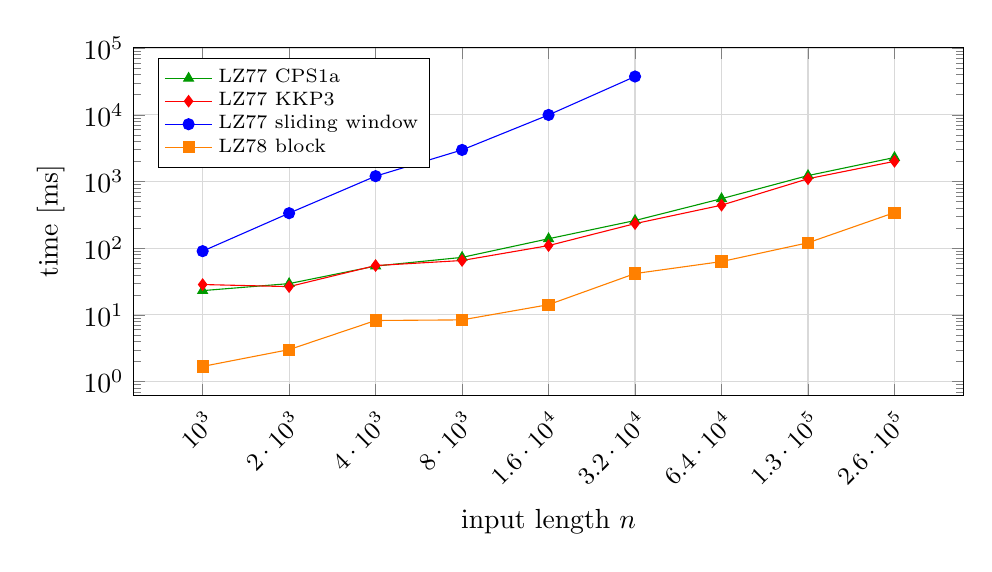
\begin{tikzpicture}
\begin{axis}[
  width = \linewidth, height = 6cm,
  xlabel = {input length $n$}, ylabel = {time [ms]},
  xmode = log, ymode = log,
  legend pos = north west, legend cell align = left,
  legend style = {font = \scriptsize, row sep = -2pt, inner sep = 2pt},
  xmajorgrids = true, ymajorgrids = true,
  xminorgrids = false, yminorgrids = false,
  minor tick num = 0,
  grid style = {draw = gray!30},
  xtick = {1000, 2000, 4000, 8000, 16000, 32000, 64000, 128000, 256000},
  xticklabels = {$10^{3}$, $2 \cdot 10^{3}$, $4 \cdot 10^{3}$, $8 \cdot 10^{3}$, $1.6 \cdot 10^{4}$, $3.2 \cdot 10^{4}$, $6.4 \cdot 10^{4}$, $1.3 \cdot 10^{5}$, $2.6 \cdot 10^{5}$},
  x tick label style = {rotate = 45, anchor = north east, font = \small},
]
\addplot[color = green!60!black, mark = triangle*] coordinates {(1000, 23.15) (2000, 29.49) (4000, 54.04) (8000, 72.95) (16000, 138.71) (32000, 260.41) (64000, 553.19) (128000, 1228.74) (256000, 2293.59)};
\addlegendentry{LZ77 CPS1a}
\addplot[color = red, mark = diamond*] coordinates {(1000, 28.57) (2000, 26.58) (4000, 54.98) (8000, 65.49) (16000, 109.56) (32000, 233.9) (64000, 442.13) (128000, 1101.65) (256000, 2008.58)};
\addlegendentry{LZ77 KKP3}
\addplot[color = blue, mark = *] coordinates {(1000, 90.41) (2000, 335.41) (4000, 1204.21) (8000, 2978.29) (16000, 9966.61) (32000, 37584.71)};
\addlegendentry{LZ77 sliding window}
\addplot[color = orange, mark = square*] coordinates {(1000, 1.69) (2000, 3.02) (4000, 8.25) (8000, 8.43) (16000, 14.25) (32000, 41.72) (64000, 63.12) (128000, 120.72) (256000, 342.32)};
\addlegendentry{LZ78 block}
\end{axis}
\end{tikzpicture}
\captionof{figure}{random binary, encoding time.}
\label{fig:random-binary-encoding}
\end{center}

\begin{center}
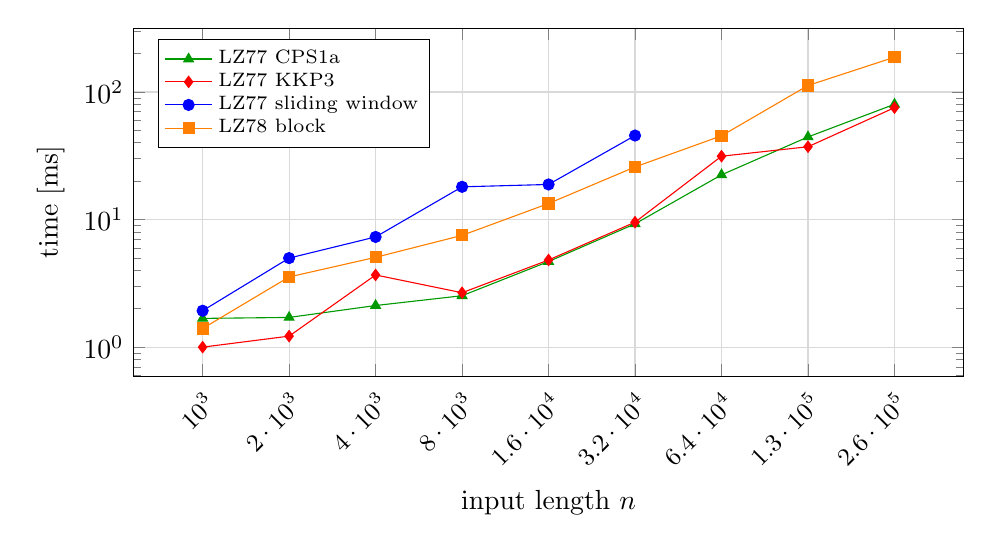
\begin{tikzpicture}
\begin{axis}[
  width = \linewidth, height = 6cm,
  xlabel = {input length $n$}, ylabel = {time [ms]},
  xmode = log, ymode = log,
  legend pos = north west, legend cell align = left,
  legend style = {font = \scriptsize, row sep = -2pt, inner sep = 2pt},
  xmajorgrids = true, ymajorgrids = true,
  xminorgrids = false, yminorgrids = false,
  minor tick num = 0,
  grid style = {draw = gray!30},
  xtick = {1000, 2000, 4000, 8000, 16000, 32000, 64000, 128000, 256000},
  xticklabels = {$10^{3}$, $2 \cdot 10^{3}$, $4 \cdot 10^{3}$, $8 \cdot 10^{3}$, $1.6 \cdot 10^{4}$, $3.2 \cdot 10^{4}$, $6.4 \cdot 10^{4}$, $1.3 \cdot 10^{5}$, $2.6 \cdot 10^{5}$},
  x tick label style = {rotate = 45, anchor = north east, font = \small},
]
\addplot[color = green!60!black, mark = triangle*] coordinates {(1000, 1.68) (2000, 1.71) (4000, 2.12) (8000, 2.53) (16000, 4.69) (32000, 9.26) (64000, 22.42) (128000, 44.45) (256000, 80.11)};
\addlegendentry{LZ77 CPS1a}
\addplot[color = red, mark = diamond*] coordinates {(1000, 1.0) (2000, 1.22) (4000, 3.68) (8000, 2.67) (16000, 4.82) (32000, 9.54) (64000, 31.38) (128000, 37.24) (256000, 75.35)};
\addlegendentry{LZ77 KKP3}
\addplot[color = blue, mark = *] coordinates {(1000, 1.93) (2000, 4.99) (4000, 7.31) (8000, 18.06) (16000, 18.85) (32000, 45.58)};
\addlegendentry{LZ77 sliding window}
\addplot[color = orange, mark = square*] coordinates {(1000, 1.4) (2000, 3.55) (4000, 5.06) (8000, 7.52) (16000, 13.36) (32000, 25.85) (64000, 45.36) (128000, 112.46) (256000, 187.37)};
\addlegendentry{LZ78 block}
\end{axis}
\end{tikzpicture}
\captionof{figure}{random binary, decoding time.}
\label{fig:random-binary-decoding}
\end{center}

\begin{center}
\begin{tabular}{lrrrrrr}
\hline
algorithm & $n$ & $\alpha$ & $z$ & $\rho$ & encode [ms] & decode [ms] \\
\hline
LZ77 sliding window & 32000 & 2 & 2175 & 2.107 & 37815.84 & 34.95 \\
LZ78 block & 32000 & 2 & 3218 & 1.1793 & 26.11 & 22.39 \\
LZ77 CPS1a & 32000 & 2 & 2175 & 1.4273 & 255.39 & 9.09 \\
LZ77 KKP3 & 32000 & 2 & 2175 & 1.4273 & 220.57 & 10.32 \\
\hline
\end{tabular}
\captionof{table}{random binary: uniform over two letters.}
\label{tab:random-binary}
\end{center}
}

\subsubsection{Pan Tadeusz}
{
\setlength{\floatsep}{6pt plus 2pt minus 2pt}
\setlength{\textfloatsep}{6pt plus 2pt minus 2pt}
\setlength{\intextsep}{6pt plus 2pt minus 2pt}
\setlength{\abovecaptionskip}{4pt}
\setlength{\belowcaptionskip}{0pt}

\begin{center}
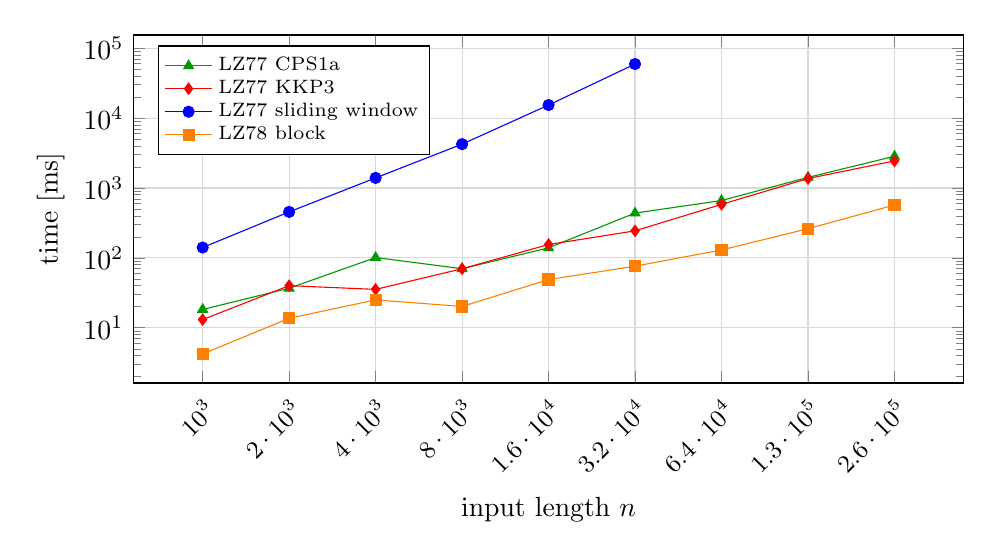
\begin{tikzpicture}
\begin{axis}[
  width = \linewidth, height = 6cm,
  xlabel = {input length $n$}, ylabel = {time [ms]},
  xmode = log, ymode = log,
  legend pos = north west, legend cell align = left,
  legend style = {font = \scriptsize, row sep = -2pt, inner sep = 2pt},
  xmajorgrids = true, ymajorgrids = true,
  xminorgrids = false, yminorgrids = false,
  minor tick num = 0,
  grid style = {draw = gray!30},
  xtick = {1000, 2000, 4000, 8000, 16000, 32000, 64000, 128000, 256000},
  xticklabels = {$10^{3}$, $2 \cdot 10^{3}$, $4 \cdot 10^{3}$, $8 \cdot 10^{3}$, $1.6 \cdot 10^{4}$, $3.2 \cdot 10^{4}$, $6.4 \cdot 10^{4}$, $1.3 \cdot 10^{5}$, $2.6 \cdot 10^{5}$},
  x tick label style = {rotate = 45, anchor = north east, font = \small},
]
\addplot[color = green!60!black, mark = triangle*] coordinates {(1000, 18.28) (2000, 36.78) (4000, 101.1) (8000, 69.96) (16000, 139.19) (32000, 437.01) (64000, 660.93) (128000, 1418.77) (256000, 2840.15)};
\addlegendentry{LZ77 CPS1a}
\addplot[color = red, mark = diamond*] coordinates {(1000, 13.09) (2000, 40.03) (4000, 35.41) (8000, 69.86) (16000, 155.27) (32000, 243.6) (64000, 582.68) (128000, 1365.72) (256000, 2436.28)};
\addlegendentry{LZ77 KKP3}
\addplot[color = blue, mark = *] coordinates {(1000, 140.51) (2000, 454.42) (4000, 1393.42) (8000, 4235.39) (16000, 15349.14) (32000, 59263.25)};
\addlegendentry{LZ77 sliding window}
\addplot[color = orange, mark = square*] coordinates {(1000, 4.22) (2000, 13.67) (4000, 25.07) (8000, 20.17) (16000, 48.93) (32000, 76.0) (64000, 129.77) (128000, 261.37) (256000, 570.51)};
\addlegendentry{LZ78 block}
\end{axis}
\end{tikzpicture}
\captionof{figure}{natural, encoding time.}
\label{fig:natural-encoding}
\end{center}

\begin{center}
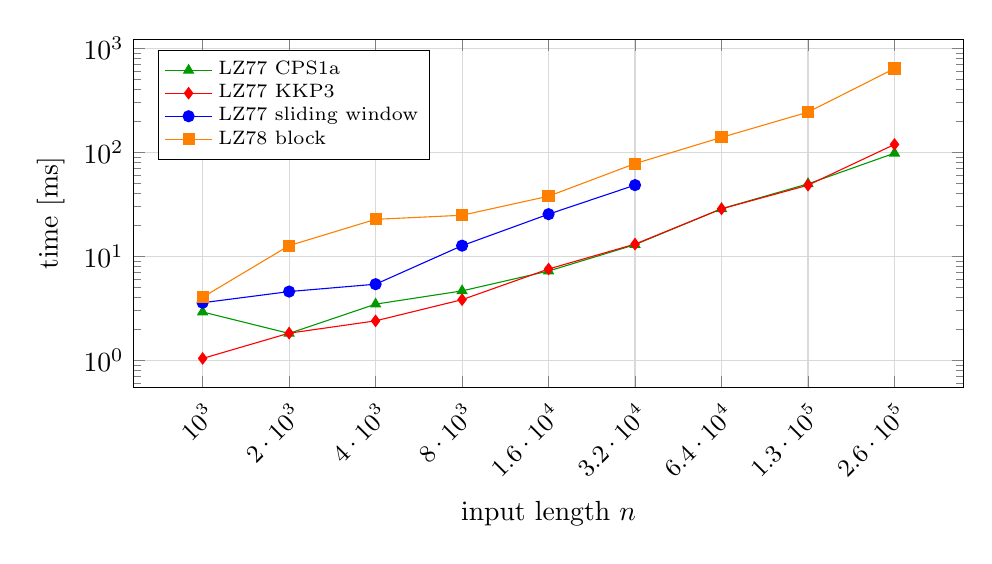
\begin{tikzpicture}
\begin{axis}[
  width = \linewidth, height = 6cm,
  xlabel = {input length $n$}, ylabel = {time [ms]},
  xmode = log, ymode = log,
  legend pos = north west, legend cell align = left,
  legend style = {font = \scriptsize, row sep = -2pt, inner sep = 2pt},
  xmajorgrids = true, ymajorgrids = true,
  xminorgrids = false, yminorgrids = false,
  minor tick num = 0,
  grid style = {draw = gray!30},
  xtick = {1000, 2000, 4000, 8000, 16000, 32000, 64000, 128000, 256000},
  xticklabels = {$10^{3}$, $2 \cdot 10^{3}$, $4 \cdot 10^{3}$, $8 \cdot 10^{3}$, $1.6 \cdot 10^{4}$, $3.2 \cdot 10^{4}$, $6.4 \cdot 10^{4}$, $1.3 \cdot 10^{5}$, $2.6 \cdot 10^{5}$},
  x tick label style = {rotate = 45, anchor = north east, font = \small},
]
\addplot[color = green!60!black, mark = triangle*] coordinates {(1000, 2.91) (2000, 1.81) (4000, 3.46) (8000, 4.64) (16000, 7.2) (32000, 12.91) (64000, 28.6) (128000, 49.59) (256000, 97.79)};
\addlegendentry{LZ77 CPS1a}
\addplot[color = red, mark = diamond*] coordinates {(1000, 1.04) (2000, 1.82) (4000, 2.39) (8000, 3.82) (16000, 7.53) (32000, 13.07) (64000, 28.51) (128000, 48.16) (256000, 118.66)};
\addlegendentry{LZ77 KKP3}
\addplot[color = blue, mark = *] coordinates {(1000, 3.57) (2000, 4.57) (4000, 5.38) (8000, 12.63) (16000, 25.35) (32000, 48.24)};
\addlegendentry{LZ77 sliding window}
\addplot[color = orange, mark = square*] coordinates {(1000, 4.03) (2000, 12.63) (4000, 22.62) (8000, 24.75) (16000, 37.74) (32000, 77.66) (64000, 138.71) (128000, 242.65) (256000, 636.97)};
\addlegendentry{LZ78 block}
\end{axis}
\end{tikzpicture}
\captionof{figure}{natural, decoding time.}
\label{fig:natural-decoding}
\end{center}

\begin{center}
\begin{tabular}{lrrrrrr}
\hline
algorithm & $n$ & $\alpha$ & $z$ & $\rho$ & encode [ms] & decode [ms] \\
\hline
LZ77 sliding window & 32000 & 34 & 6133 & 1.3416 & 55752.28 & 47.67 \\
LZ78 block & 32000 & 34 & 8078 & 0.8481 & 64.83 & 65.97 \\
LZ77 CPS1a & 32000 & 34 & 6133 & 0.9583 & 314.13 & 12.97 \\
LZ77 KKP3 & 32000 & 34 & 6133 & 0.9583 & 281.1 & 25.07 \\
\hline
\end{tabular}
\captionof{table}{natural: Pan Tadeusz, letters and spaces only.}
\label{tab:natural}
\end{center}
}

\subsection{Results summary}

The sliding-window LZ77 deserves a separate remark. Run offline, as all the experiments are, it has \(L_s = \len{S}\), so its length field is as wide as the pointer field and every codeword carries \(1 + 2\ceil{\log_\alpha\len{S}}\) symbols instead of \(1 + \ceil{\log_\alpha \len{S}} + \ceil{\log_\alpha (\max_i l_i + 1)}\) of CPS1a and KKP3 which size the length field from the factors actually produced. The number of factors is identical --- \(z\) agrees with CPS1a and KKP3 in every table, so the worse ratio is entirely an artifact of its implementation for rather online usage. What the tables really show about this implementation is its running time: since with the window equal to the whole text the naive search of \textsc{ReproducibleExtension} (see \Cref{def:reproducible-extension}) becomes up to quadratic.

\paragraph{The number of factors and the compression ratio.}
On the compressible texts: Fibonacci, Thue-Morse and the run of one closed letter, the three LZ77 variants produce the same factorization and the same small number of factors, while LZ78 produces a lot more factors what is caused by \emph{incremental parsing}, which doesn't support long overlapping factors. The gap is very big because of the property that LZ78 does not allow overlapping in the process of factor production. The three LZ77 implementations agree on \(z\) in every table, as they must, since they compute the same factorization by three different routes.

On the incompressible (have small average factor length) texts the picture reverses, the gradually increasing codeword length covers the loss in incremental parsing. Note that it is natural, that we get a ratio greater than 1, because in such cases we face the problem, that the length of codeword eats away any possible gain in encoded representation in both LZ77 and LZ78 approaches. 
% It is easy to see, that in our algorithms the number of factors and the compression ratio has inseparably linked forms of behavior.

\paragraph{The encoding time.}
What the tables really show about the sliding-window implementation is its running time, and here it is worth being precise about when it is slow, because it is not slow everywhere. Its cost is not driven by the length of the source alone but by the type of text itself: on one type it can run in almost \(\Theta(n)\) time, like in \emph{Fibonacci} (see \Cref{tab:Fibonacci}), on the other type it will cost \(\Theta(n^{1.5})\) or more, like in \emph{random-26} (see \Cref{tab:random-26}). Overall \emph{CPS1a} and \emph{KKP3} pay for not small amount of additional structures on all types of text, so their additional constant in complexity makes them slower than \emph{LZ78}.

\paragraph{The decoding time.}
Decoding behaves as expected, LZ78 runs slower due to the greater amount of factors. \emph{CPS1a} and \emph{KKP3} decode fastest everywhere although they share the decoder with the sliding window implementation and parse the same triples. The difference is that the latter reconstructs the output inside a ring buffer, so every symbol access requires a lot of jumps in memory, while the originally offline variants copy from the output built so far.

% Decoding behaves as expected, LZ78 runs slower due to greater amount of factors.

\paragraph{Implementation details}
In \emph{CPS1a} we use \(\mathrm{SA}\) (in \emph{KKP3} too) and \(\mathrm{LCP}\) of Definitions \ref{def:suffix-array} and \ref{def:lcp-array}. Both are already available in the repository and we use them as they are, rather than reimplementing them: SA is built by induced sorting, the algorithm of \cite{nong2009}, and \(\mathrm{LCP}\) by the linear-time method of \cite{kasai2001}.